\documentclass[UTF8,11pt,a4paper]{ctexart}
\usepackage[margin=2.3cm,headheight=15pt]{geometry}
\usepackage{amsmath,amssymb,bm,booktabs,longtable,tabularx,multirow,array,graphicx,float,caption,subcaption,enumitem,fancyhdr,hyperref,xcolor,listings,lastpage}
\hypersetup{colorlinks=true,linkcolor=black,citecolor=black,urlcolor=blue}
\setlength{\parindent}{2em}
\setlength{\parskip}{0.15em}
\linespread{1.22}
\pagestyle{fancy}
\fancyhf{}
\fancyhead[C]{2026年度“策联杯”数学建模精英联赛 C题}
\fancyfoot[C]{\thepage}
\renewcommand{\headrulewidth}{0.4pt}
\captionsetup{font=small,labelsep=quad}
\newcommand{\mm}[1]{\ensuremath{#1}}
\newcommand{\clip}{\operatorname{clip}}
\newcommand{\norm}[1]{#1^{\prime}}
\lstset{basicstyle=\ttfamily\scriptsize,breaklines=true,frame=single,numbers=left,numberstyle=\tiny,showstringspaces=false,columns=fullflexible,keepspaces=true,tabsize=4}
\title{\vspace{-1.8cm}\textbf{足球世界杯赛事预测与赛程资源协同优化}\\[0.3em]\large 时序集成、混合整数规划与同截面动态重配置}
\author{}
\date{}

\begin{document}
\thispagestyle{fancy}
\maketitle
\vspace{-1.4cm}
\begin{abstract}
本文针对48队、12组、72场模拟世界杯，建立“赛前需求预测--场馆时段协同--赛中反馈重配置--现实赛程对照”的闭环。首先严格保持官方日期划分，排除比分、xG、射门、控球和实际上座等赛后泄漏变量，以球队实力、球迷基础、市场隐含概率、赛事阶段和时区配对构造赛前特征；通过五折时间阻断验证比较岭回归、极端随机树、随机森林与直方图梯度提升，再用非负最小二乘集成。集成的OOF MSE为243.51（百万人）$^2$、RMSE为15.60百万人；权重在同一OOF预测上拟合和评价，并非嵌套外层验证。隐藏测试标签不可见，故该结果仅为内部时序证据。最终给出140条测试预测及72场模拟比赛预测，后者范围为1.499--1.985亿人。

其次，以比赛--场馆--时段二元变量建立混合整数规划。我们按官方公式计算票务、转播、悬念、吸引力、完整成本、旅行、公平和原值风险，并把逐队相邻轮次60小时约束直接写入模型。21,420个轮次日期预筛候选经HiGHS有界求解得到目标值0.275364的可执行方案：最小休息81小时，球队黄金时段次数为1--2，大容量场馆次数全部为1，场馆总承办量为2--8。求解在300秒停止，预筛模型最优性缺口3.06\%；该界不覆盖未预筛题面可行域，故仅主张预筛模型内“可行近优”。

再次，利用前两轮同一信息截面更新球队状态和泊松进球均值，联合模拟24场第三轮比赛20,000次，并对积分、净胜球、进球数完全相同情形实施等比例晋级权重。每次仿真的晋级权重总和均为32。静态与动态资源方案在相同候选集、容量、预算及更新后评价口径下比较；票务、转播、成本共享Min--Max边界，吸引力和风险直接使用官方$[0,1]$原值。两者均求得全局最优。动态总净效益由7.16063升至7.17587（+0.2129\%），主要以票务价值下降0.59\%换取转播价值上升0.07\%和资源成本下降3.55\%；这只是给定模型实例内的信息价值。

最后，从FIFA官方接口采集2022卡塔尔世界杯48场小组赛。除11项分项诊断外，按Q2八项定义、共同边界和官方权重计算代理总分：2022实际为0.17710，模拟优化为0.19163。对实际赛程缺失的吸引力、成本、旅行时间和风险代理执行81组敏感性时，优化减实际的分差范围为$-0.04048$至$0.04542$并发生排序翻转。因此基准代理下模拟方案仅略高，不能据此声称总体、机制或因果优越；分项差异仍须单独呈现。

\textbf{关键词：} 转播需求预测；时间阻断验证；混合整数规划；泊松仿真；动态资源配置；赛程公平
\end{abstract}
\newpage

\section{问题重述与研究思路}
赛事组织者需要在不可同时满足的商业、竞技和执行目标之间作出可审计选择。问题一要求从历史比赛预测转播观看人数；问题二把预测嵌入72场比赛的场馆--时段联合分配；问题三在固定第三轮赛程下使用前两轮反馈重新配置转播、安保、交通和票价；问题四要求把模拟最优方案置于真实世界杯约束中解释。

本文不把四问割裂：问题一的预测作为问题二、三的需求基线；问题二的场馆和时段固定问题三的容量与日期；问题三的同截面仿真避免第三轮信息串扰；问题四用真实赛程揭示模拟目标未覆盖的制度与地理约束。所有随机过程固定种子20260830，所有输出由同一代码链产生。

\section{数据审计、假设与符号}
\subsection{数据审计}
官方工作簿含15张表。历史比赛700场，其中训练集560场（2018-01-12至2024-07-27），测试集140场（2024-08-05至2025-12-28）；唯一系统性缺失是测试集目标 \texttt{tv\_viewers}。对阵表包含72个唯一比赛编号；16个场馆的最小总承办量均为2、最大为8；80个时段覆盖2026-06-11至06-30；动态反馈恰含前两轮48场。输出模板的字段名、顺序和单位被视为硬约束。

\subsection{基本假设}
\begin{enumerate}[label=H\arabic*.]
\item 官方附件中的球队属性、距离、风险、容量和价格参数在模拟赛期内有效；模拟属性不解释为FIFA官方评级。
\item 问题一只使用开球前可知信息。历史赛后统计不用于测试预测，避免目标泄漏。
\item 问题二把三个轮次分别预筛到06-11--15、06-18--22、06-26--30；这是透明的运营缓冲策略，并非题目新增事实。逐队轮次先后和60小时休息已显式进入MILP，并在输出后再次重算。
\item 问题三24场第三轮比赛共享前两轮结束时的信息截面；任何一场第三轮结果都不更新其他场参数。
\item 问题四按场、按球队相邻比赛转移或比例指标标准化赛事规模；Q2八项总分使用两赛事共同边界。FIFA接口缺失的容量以整届赛事该场馆最大官方上座代理，U/H/C/D/R缺口使用可审计代理并另做敏感性分析。
\end{enumerate}

\subsection{主要符号}
\begin{table}[H]\centering\small
\begin{tabularx}{\textwidth}{cXcX}
\toprule
符号 & 含义 & 符号 & 含义\\\midrule
$m,v,s$ & 比赛、场馆、时段 & $x_{mvs}$ & 是否将$m$分配至$(v,s)$\\
$T,B,U,H$ & 票务、转播、悬念、吸引力 & $C,D,F,R$ & 成本、旅行、公平、风险\\
$S_t,h_t$ & 球队状态、伤病影响 & $p_t,Q_i$ & 晋级概率、比赛晋级重要性\\
$N_i,V_i$ & 最终现场、转播需求 & $c_i^B,c_i^S,c_i^T$ & 三类资源成本指数\\
\bottomrule
\end{tabularx}
\end{table}

\section{问题一：转播观看人数预测}
\subsection{特征工程与泄漏控制}
先将十进制赔率转换为去除庄家边际的三项隐含概率
\begin{equation}
p_k=\frac{o_k^{-1}}{o_a^{-1}+o_d^{-1}+o_b^{-1}},\quad k\in\{a,d,b\},
\end{equation}
并构造归一化熵 $-\sum_k p_k\log p_k/\log3$、悬念 $1-\max_kp_k$。球队层面使用双方Elo与排名的均值/差，市场价值、球星、球迷、攻防风格和综合实力的均值/最大值/差，以及洲际足联配对、时区区域配对、东道主和中立场标记；赛事层面使用赛事类别、阶段和年份趋势。

实际比分、xG、射门、控球、实际上座均发生在赛后，虽然训练表可见，但全部排除。72场未来赛没有赔率时，以附件基准胜/平/负概率构造等价赔率；仍保留世界杯、小组赛、中立场等赛前语义。

\subsection{时间阻断集成}
训练样本按日期排序，用五个扩展窗执行时间阻断验证。候选模型分别捕捉线性外推和非线性交互，其中随机森林用于表征非线性特征交互\cite{breiman}。设第$j$个模型预测为 $\hat y_j$，在所有OOF记录上求
\begin{equation}
\min_{w_j\ge0}\sum_i\left(y_i-\sum_jw_j\hat y_{ij}\right)^2,
\qquad \sum_jw_j=1.
\end{equation}
得到岭回归、极端随机树、随机森林权重分别为0.4877、0.2705、0.2418，梯度提升权重为0。非负约束减少不稳定抵消。

\begin{figure}[H]\centering
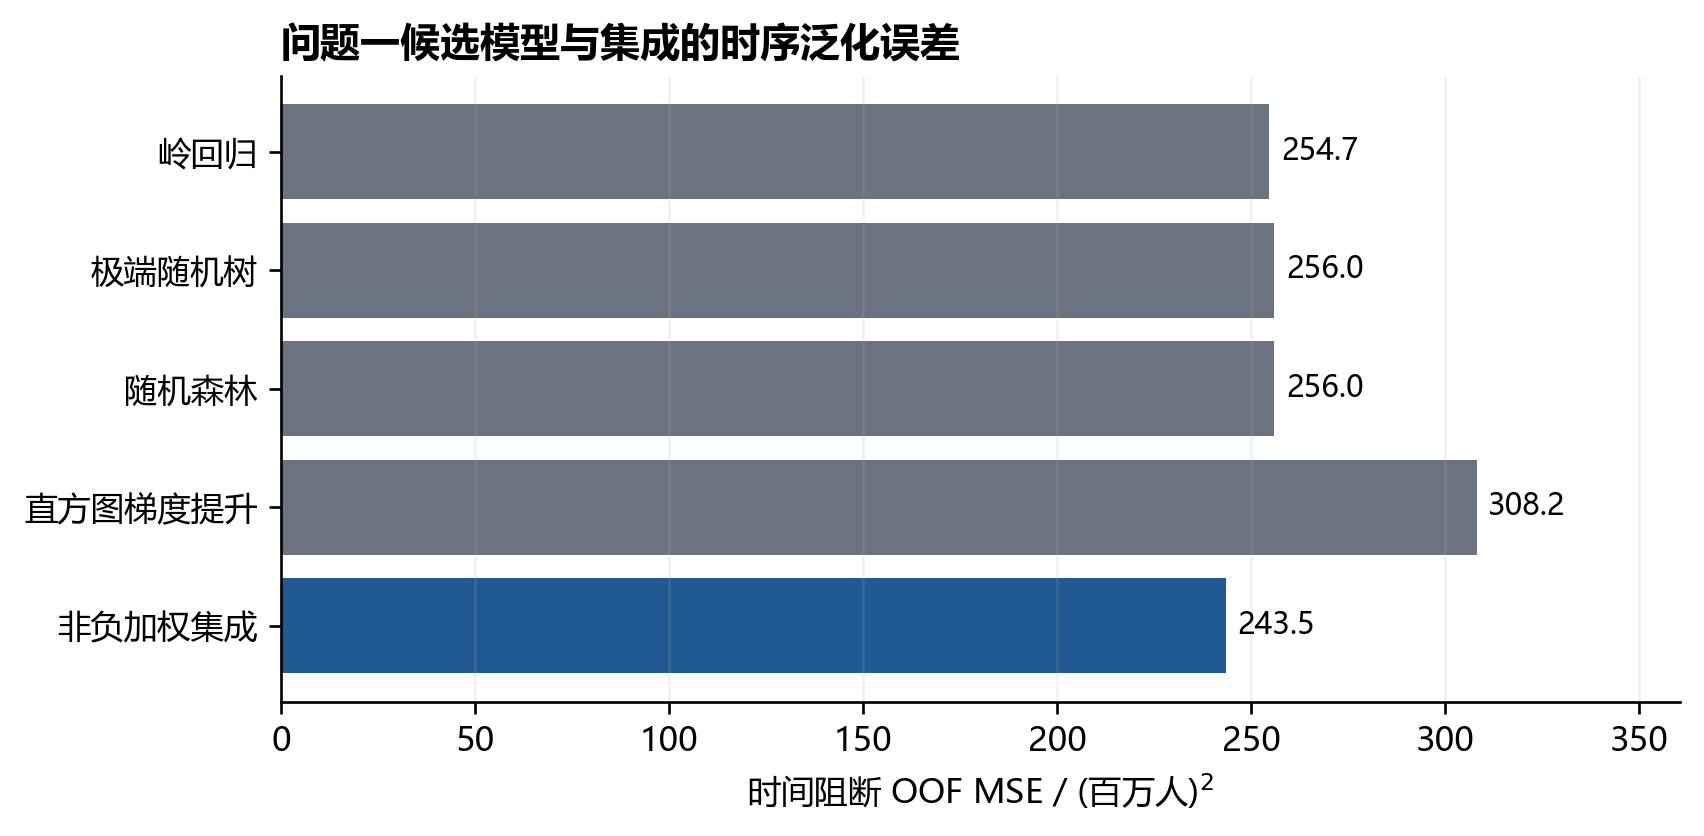
\includegraphics[width=0.84\textwidth]{../figures/q1_model_cv.png}
\caption{候选模型与集成的时间阻断OOF误差}
\end{figure}

\begin{table}[H]\centering\small
\begin{tabular}{lrr}
\toprule 模型 & OOF MSE/（百万人）$^2$ & 相对集成劣化\\\midrule
岭回归 & 254.72 & 4.60\%\\
极端随机树 & 256.02 & 5.14\%\\
随机森林 & 255.98 & 5.12\%\\
直方图梯度提升 & 308.16 & 26.55\%\\
非负集成 & \textbf{243.51} & --\\\bottomrule
\end{tabular}
\end{table}

最近一折（2023-07-29至2024-07-27）岭回归MSE为175.31，明显低于最早一折的346.03，说明扩展训练窗有益。最终在560场训练集重训并输出测试预测113.17--188.04百万人；72场未来小组赛预测为149,924,516--198,544,722人。由于测试真值隐藏，不能报告官方测试MSE。

\section{问题二：场馆与开球时段协同优化}
\subsection{候选指标}
对每个满足场馆安保能力的$(m,v,s)$计算；风险识别和按比赛风险配置安保资源遵循赛事安全管理的一般原则\cite{fifasec}：
\begin{align}
T_{mvs}&=P_r\min(N_m^{0},K_v),\\
B_{mvs}&=\hat V_m u_r g_s w_r,\\
C_{mv}&=c_v^{op}+0.1\,q_m c_v^{sec},\\
R_{mv}&=0.5r_v^{clim}+0.3\frac{\min(N_m^0,K_v)}{K_v}+0.2\frac{q_m}{Q_v}.
\end{align}
其中金额成本以百万美元计，因此10万美元写为0.1百万美元。所有16个场馆的最小承办量均为2，故总启用成本17.95百万美元在可行域内恒定；实现将其按72场均摊到$C_{mv}$后再归一化，完整成本仍在结果中单列。

旅行负担先在全部距离记录上分别对距离、时间、时区差做Min--Max，再按$0.5,0.3,0.2$合成。第一轮由球队代表地到候选场馆；第二、三轮严格按题意，将上一轮所有安保合格场馆作为可能起点，取到当前场馆的平均负担；双方再平均。

票务$T$、转播$B$、完整成本$C$和旅行$D$以全部预筛可行候选的上下界归一化：
\begin{equation}
z'=\begin{cases}(z-z_{\min})/(z_{\max}-z_{\min}),&z_{\max}>z_{\min},\\0,&\text{否则}.\end{cases}
\end{equation}
悬念$U$直接使用附件$[0,1]$原值，吸引力$H$除以100，执行风险$R$按官方约定直接使用原值$[0,1]$，不再二次Min--Max。悬念和吸引力仅依赖比赛，因而影响整套方案的报告值但不改变同一比赛的场馆--时段排序。

\subsection{MILP约束}
核心变量 $x_{mvs}\in\{0,1\}$。比赛唯一性为 $\sum_{v,s}x_{mvs}=1$；场馆--UTC冲突和转播容量分别为
\begin{equation}
\sum_mx_{mvs}\le1,\qquad \sum_{m,v}x_{mvs}\le b_s.
\end{equation}
同一场馆当地日负荷不超过 $d_v^{\max}$，阶段总量位于 $[L_v,U_v]$。对球队$t$相邻两轮比赛$m,m'$，利用时段UTC数值线性表达休息：
\begin{equation}
\sum_{v,s}\tau_s x_{m'vs}-\sum_{v,s}\tau_sx_{mvs}\ge60\ \text{小时}.
\end{equation}
第三轮高安保需求逐日受限。另引入黄金时段、大容量场馆次数的最大/最小变量，把
\begin{equation}
F=\frac12\frac{g_{\max}-g_{\min}}3+\frac12\frac{\ell_{\max}-\ell_{\min}}3
\end{equation}
线性加入目标，并硬约束 $g_{\max}-g_{\min}\le2$。

最终最大化题目基准目标
\begin{equation}
Z_2=0.25T'+0.25B'+0.15U+0.10H-0.08C'-0.07D'-0.06F-0.04R.
\end{equation}

\subsection{求解结果与可执行性}
预筛后有21,420个候选二元变量和1,642行线性约束，其中96行显式约束48队的两次相邻轮次休息。HiGHS\cite{highs}在300秒内获得可行整数解；目标0.27536440，最佳界对应相对缺口3.0570\%。该缺口只界定轮次日期预筛后的MILP，不界定未预筛原题；也不应解释成解误差一定为3.0570\%。

\begin{table}[H]\centering\small
\begin{tabular}{lrlr}
\toprule 指标 & 结果 & 指标 & 结果\\\midrule
最小相邻轮次休息 & 81 h & 场馆总承办量范围 & 2--8\\
黄金时段次数范围 & 1--2 & 大容量场馆次数范围 & 1--1\\
总票务收入 & 2.8591亿美元 & 总转播价值 & 3.3599亿美元\\
场馆启用成本 & 1,795万美元 & 运营及安保成本合计 & 3,495.5万美元\\
完整成本 & 5,290.5万美元 & 预筛模型MIP gap & 3.0570\%\\
\bottomrule
\end{tabular}
\end{table}

八项目标指标为 $T'=0.3746,B'=0.4958,U=0.4614,H=0.6397,C'=0.4358,D'=0.1994,F=0.1667,R=0.4148$。图\ref{fig:q2load}显示负荷分布；所有16个场馆被启用，低容量场馆满足最低承办量，高容量场馆承担更多比赛。
\begin{figure}[H]\centering
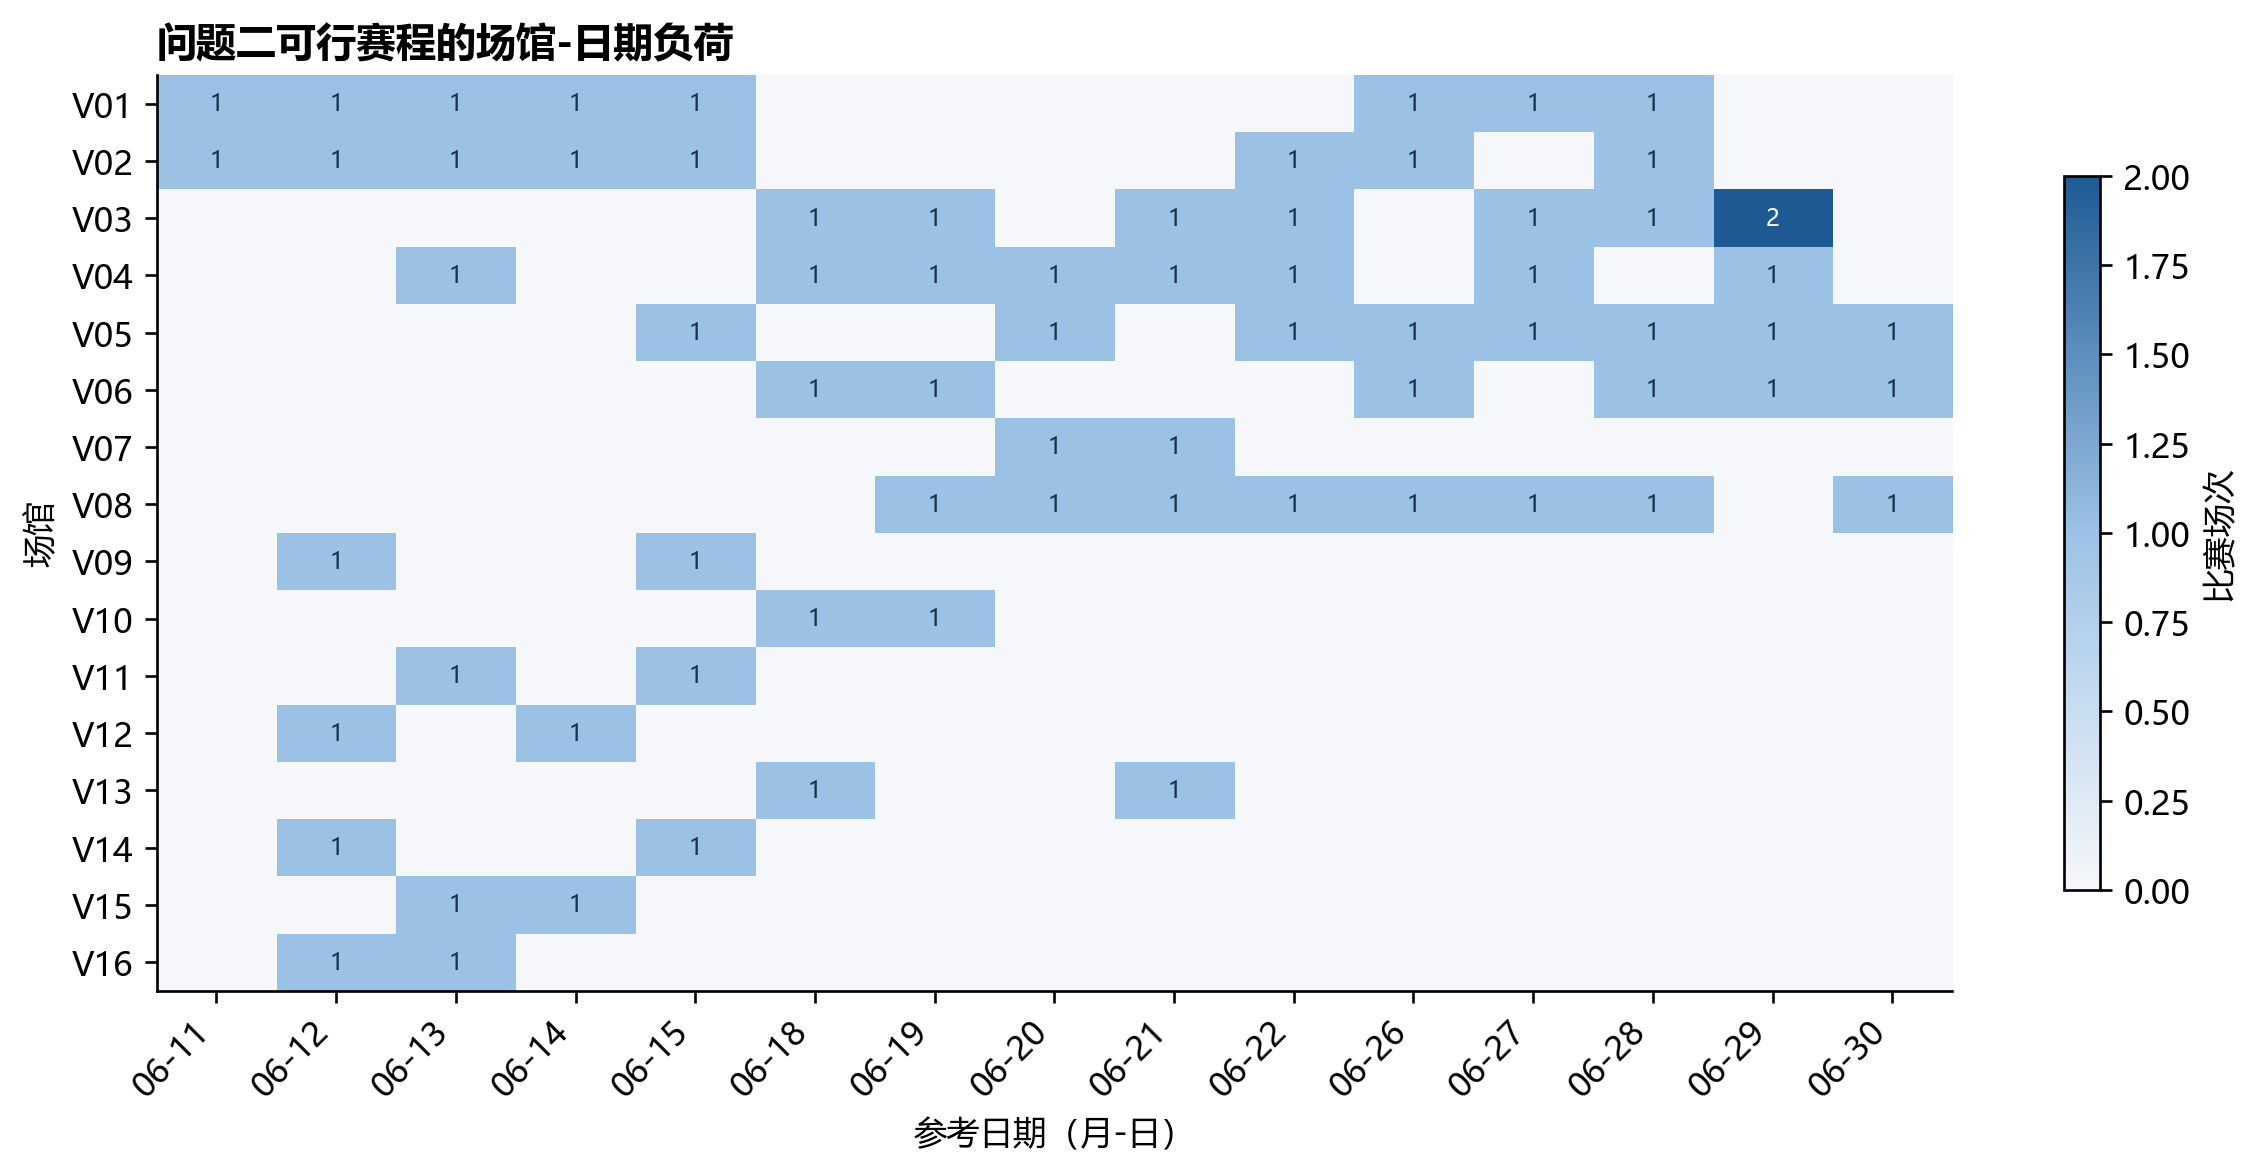
\includegraphics[width=0.96\textwidth]{../figures/q2_venue_date_load.png}
\caption{优化赛程的场馆--日期负荷}\label{fig:q2load}
\end{figure}

\section{问题三：前两轮反馈下的第三轮动态优化}
\subsection{同截面状态更新}
对球队$t$，完全按题面定义
\begin{equation}
S_t=0.45\frac{P_t}{3G_t}+0.35\left[0.5+0.5\tanh\left(\frac{(xGF_t-xGA_t)/G_t}{1.25}\right)\right]+0.20e^{-0.55RC_t/G_t}.
\end{equation}
伤病 $h_t$ 为两场平均。采用足球比分泊松建模思路\cite{dixon}，令 $\Delta_i=0.32(S_a-S_b)-0.055(h_a-h_b)$，则
\begin{equation}
\lambda_{ia}=\clip(\lambda^0_{ia}e^{\Delta_i-0.04h_a},0.15,4.50),\quad
\lambda_{ib}=\clip(\lambda^0_{ib}e^{-\Delta_i-0.04h_b},0.15,4.50).
\end{equation}

20,000次仿真同时抽取24场比分。组内按积分、净胜球、进球数排序；若分界处完全同分，设并列块大小为$b$、尚余名额为$k$，则块内每队获得$k/b$晋级权重。组内第三名身份同理，再对12个第三名竞争8席执行一次等比例分配。由此每次仿真的晋级权重严格守恒为32；由伯努利方差上界\cite{ross}，任意单队概率的理论最大Monte Carlo标准误不超过
\begin{equation}
\sqrt{0.25/20000}=0.00354.
\end{equation}

晋级重要性、反馈几何平均、更新吸引力、现场/转播需求、无激励与默契风险均依题面公式实现。特别地，条件概率 $P(\text{晋级}\mid\text{本场平/胜})$ 来自同一批联合仿真筛选，而不是重新引入其他第三轮结果。

\subsection{静态与动态公平比较}
票价需求采用常弹性形式\cite{openstax}。候选决策包含转播1--3级、安保从最低需求至场馆能力、交通1--3级、逐日允许的0.01步长票价调整，共12,546条。静态方案只用赛前需求、赛前吸引力和 $1-U$ 无激励风险优化；随后固定其决策，在更新环境中重算。动态方案用更新信息重新优化。两者评价时共享更新环境中$TV,BV,C$的Min--Max上下界；$A,R$均直接使用官方$[0,1]$原值，避免二次标准化和“各自归一化”制造虚假改善。

\begin{equation}
Z_3=\sum_{i\in I_3}\left(0.35TV_i'+0.35BV_i'+0.10A_i-0.10C_i'-0.10R_i\right).
\end{equation}
两个MILP均在根节点达到gap=0。动态总净效益提高0.2129\%；这只说明给定泊松、反馈、候选动作和效用模型的本实例中重优化略优，不能外推为现实信息的因果价值。

\begin{figure}[H]\centering
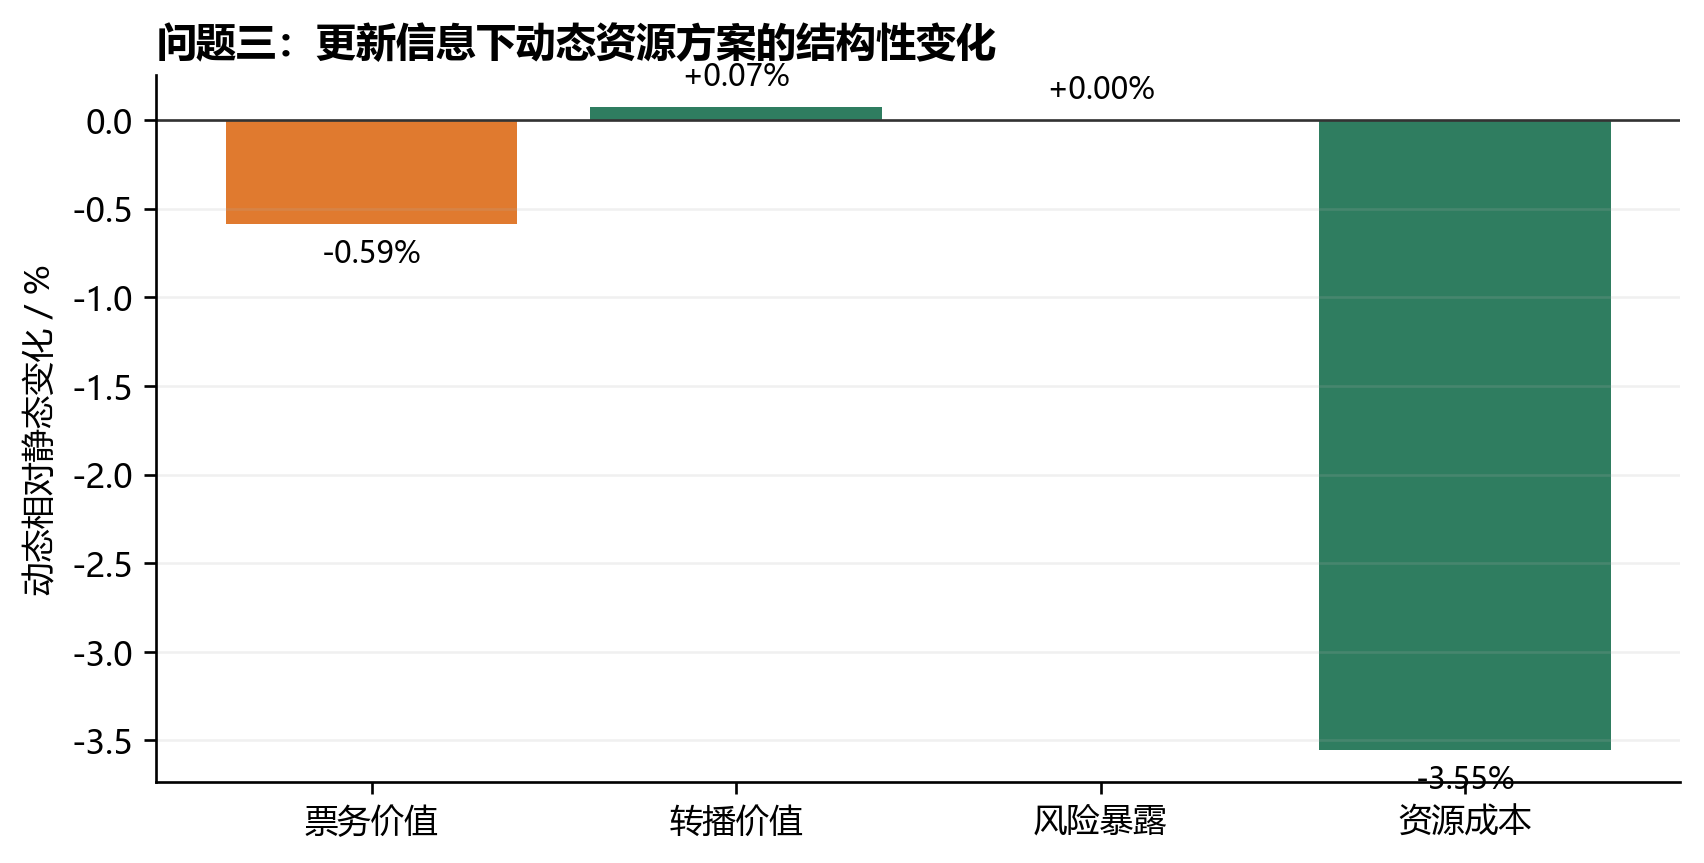
\includegraphics[width=0.82\textwidth]{../figures/q3_dynamic_vs_static.png}
\caption{动态方案相对静态固定方案的指标变化}
\end{figure}

\begin{table}[H]\centering\small
\begin{tabular}{lrrr}
\toprule 指标 & 静态固定决策（更新后评价） & 动态重优化 & 变化\\\midrule
票务价值/美元 & 113,199,288 & 112,536,082 & $-0.586\%$\\
转播价值/美元 & 166,929,088 & 167,049,223 & $+0.072\%$\\
平均风险暴露 & 0.467830 & 0.467830 & $0.000\%$\\
资源成本指数 & 366 & 353 & $-3.552\%$\\
总净效益 & 7.160628 & 7.175872 & $+0.2129\%$\\
\bottomrule
\end{tabular}
\end{table}

风险均值相同不表示逐场风险完全不变，而是当前容量和最低安保约束下，最优安保组合未改变整体均值。动态方案少投入13个成本指数，以轻微票务让渡换取转播提升。

\section{问题四：与2022卡塔尔世界杯实际赛程比较}
\subsection{数据采集与统一口径}
选择已结束且采用四队小组、每队三场的2022卡塔尔世界杯。FIFA官方接口\cite{fifaapi}提供64场赛事记录，筛选具有Group A--H标识的48场小组赛，按各组六场的UTC顺序每两场划为一轮。场馆坐标通过OpenStreetMap Nominatim\cite{nominatim}获取。实际容量代理为整届赛事中该场馆的最大FIFA官方上座；这能保持可复现，但不是建筑核定容量。

由于实际赛程48场、模拟赛程72场，金额和观众均按每场比较；旅行、休息和跨时区按每支球队两次相邻轮次转移比较；场馆利用用承办量变异系数；公平性仍用每队黄金时段和大容量场馆次数极差。Q2八项评价中，$T,B,C$在合并后的48+72条逐场记录上冻结共同Min--Max边界，$D$在两赛事相邻转移的距离、时间、时区分项上冻结共同边界，$U,H,R$按$[0,1]$原值聚合。实际$U$取Elo胜平负概率的$1-\max p$；$H$用官方72场的$U$与赛前球队属性桥接；$C$用候选场馆中位成本；$D$的卡塔尔旅行时间取$0.5+\text{距离}/60$；$R$沿用气候/安保中位数与实际上座率代理。六支缺失球队属性以训练中位数插补，故总分是可审计情景而非事实评价。

\subsection{结果与解释}
\begin{table}[H]\centering\scriptsize
\begin{tabular}{lrrl}
\toprule 指标 & 2022实际 & 模拟优化 & 优势方\\\midrule
平均每次转场距离/km & 18.9891 & 2060.2604 & 实际\\
平均休息/h & 97.8125 & 175.1875 & 优化\\
每队跨时区次数 & 0.000000 & 1.708333 & 实际\\
场馆负荷变异系数 & 0.00000000 & 0.63828474 & 实际\\
平均容量匹配率 & 0.96211634 & 0.61021250 & 实际（目标0.90）\\
黄金时段比赛占比 & 0.66666667 & 0.62500000 & 实际\\
每场观众 & 51,188.73 & 41,746.42 & 实际\\
每场票务价值/美元 & 4,869,992.40 & 3,970,978.75 & 实际\\
每场转播价值/美元 & 4,019,003.96 & 4,666,641.84 & 优化\\
公平性惩罚 & 0.83333333 & 0.16666667 & 优化\\
执行风险代理 & 0.49946823 & 0.41477674 & 优化\\
\bottomrule
\end{tabular}
\end{table}

\begin{table}[H]\centering\scriptsize
\begin{tabular}{lrrr}
\toprule Q2指标（共同口径） & 权重 & 2022实际 & 模拟优化\\\midrule
$T'$票务 & $+0.25$ & 0.3403 & 0.2110\\
$B'$转播 & $+0.25$ & 0.3517 & 0.4570\\
$U$悬念 & $+0.15$ & 0.4736 & 0.4614\\
$H$吸引力 & $+0.10$ & 0.6697 & 0.6397\\
$C'$完整成本代理 & $-0.08$ & 0.7692 & 0.5141\\
$D'$相邻转移负担代理 & $-0.07$ & 0.0344 & 0.5837\\
$F$公平惩罚 & $-0.06$ & 0.8333 & 0.1667\\
$R$风险代理 & $-0.04$ & 0.4995 & 0.4148\\\midrule
官方权重综合分 & -- & 0.17710 & 0.19163\\
\bottomrule
\end{tabular}
\end{table}

\begin{figure}[H]\centering
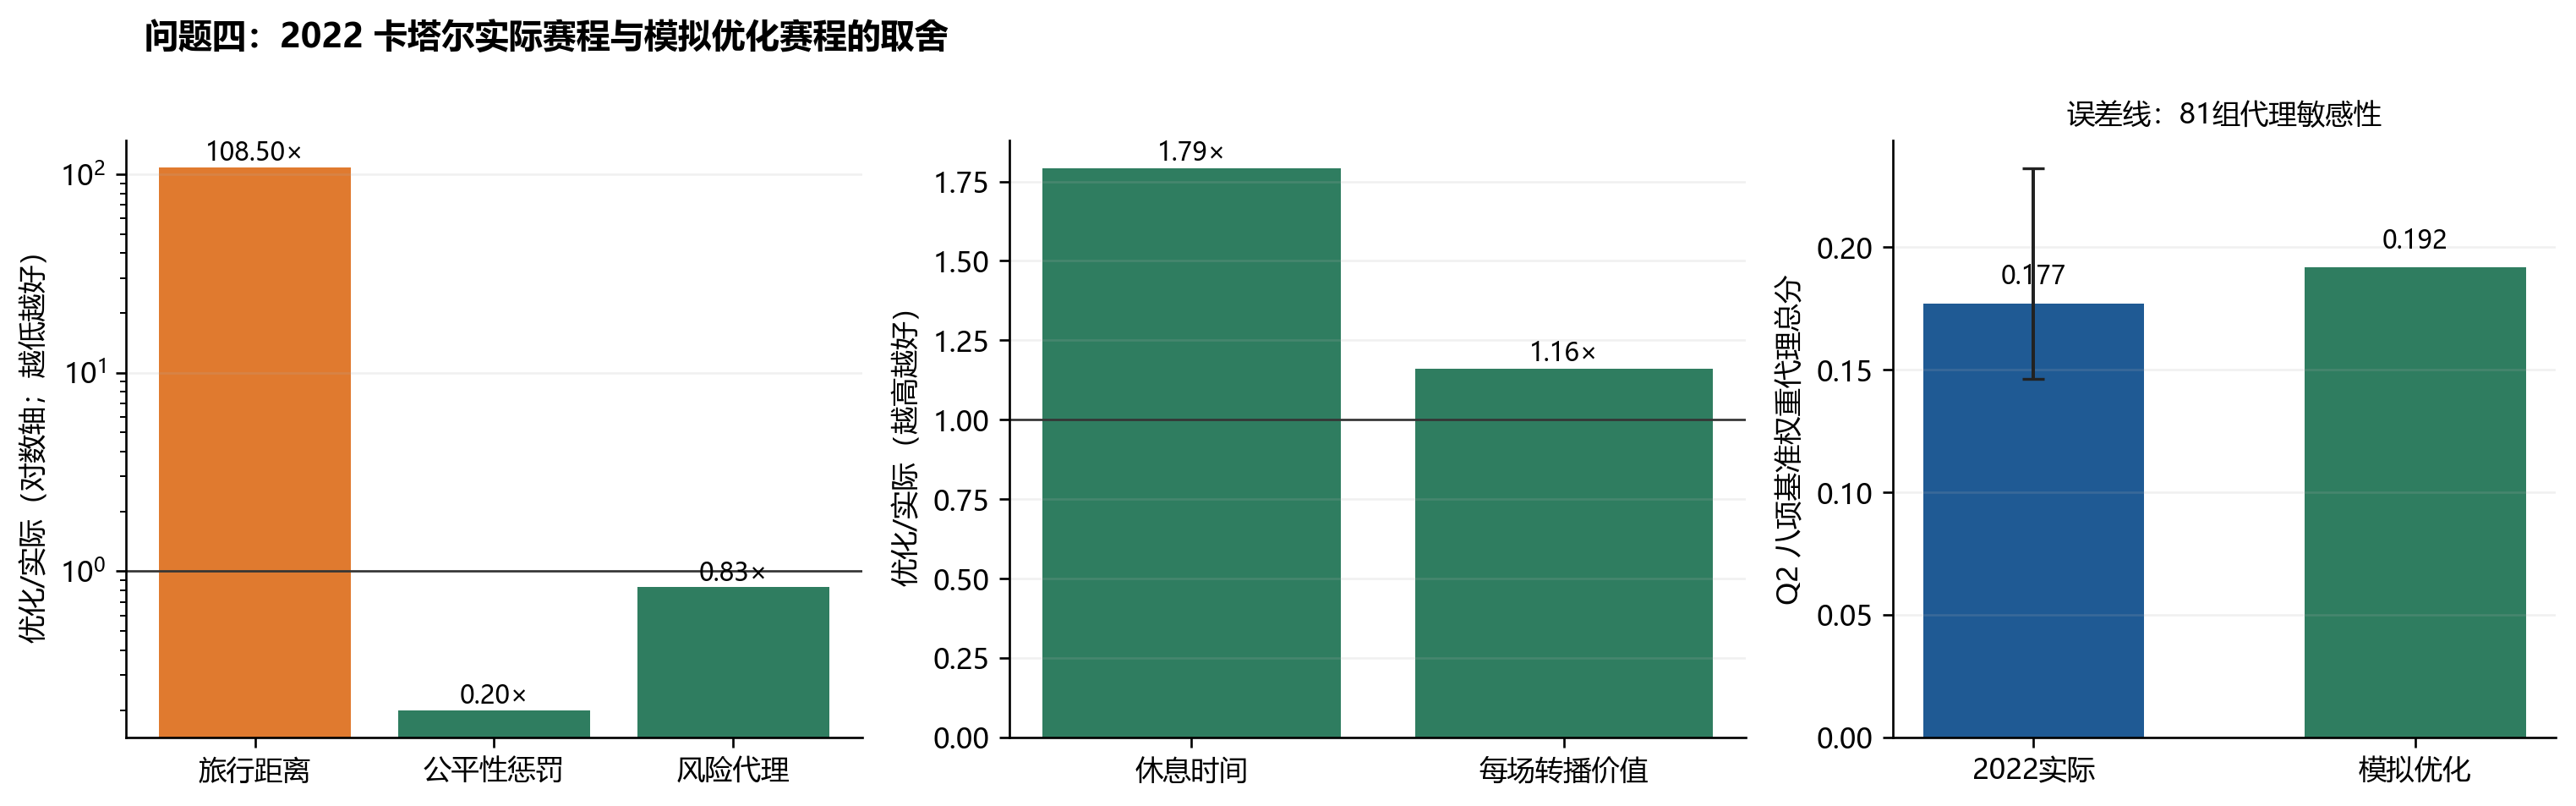
\includegraphics[width=0.95\textwidth]{../figures/q4_tradeoffs.png}
\caption{11项分项取舍与Q2八项基准权重代理总分；总分误差线来自81组代理敏感性}
\end{figure}

基准代理总分中模拟方案高0.01452。对成本乘数0.75--1.25、吸引力平移$\pm0.08$、风险平移$\pm0.10$和卡塔尔旅行速度40--80 km/h枚举81组冻结边界敏感性，得到
\[
\Delta Z=Z_{\rm optimized}-Z_{\rm actual}\in[-0.04048,\ 0.04542],
\]
排序发生翻转。因此总分结论不稳健，只能与11项诊断并列报告。实际赛程在旅行、场馆均衡和容量匹配上占优，模拟方案在休息、公平、转播和风险代理上占优；这些是披露代理下的算术差异，不证明举办地理的因果机制。现实赛程还受末轮同时开球、城市交通、电视合同和安保隔离等未入模约束。

\section{稳健性、机械核验与局限}
\subsection{有判别力的检查}
\begin{enumerate}
\item \textbf{预测：} 五折严格向前验证；集成相对最佳单模型MSE下降4.40\%；最近一折误差低于早期折。集成权重与误差来自同一OOF记录而非嵌套外层；隐藏测试真值不可见。
\item \textbf{赛程：} 逐条重算72个唯一比赛、场馆--UTC不冲突、转播容量、当地日负荷、场馆总量、安保资格、逐队轮次与休息；最小休息81小时。风险原值口径、恒定启用成本与96条休息约束另作机械复核。
\item \textbf{仿真：} 20,000次中每次晋级权重和为32；概率范围0.00266--1.00000；条件样本计数随工件保存。静态和动态的资源容量、预算、票价边界逐日重算，动态总目标不低于固定静态方案。
\item \textbf{外部数据：} FIFA原始JSON、Nominatim响应、URL和访问日均保存；48场结构、11项诊断、Q2八项权重总分、共同边界和81组敏感性均写入机器可读审计。
\end{enumerate}

\subsection{局限与不能推出的结论}
\begin{itemize}
\item 问题一训练样本仅560场，且附件可能是模拟数据。OOF集成评价非嵌套，不能外推为真实世界杯收视精度或隐藏测试官方得分。
\item 问题二使用透明轮次日期预筛且在300秒停止，3.0570\% gap只属于预筛模型；启发式日期缓冲可能排除未预筛域中的更优解。
\item 问题三泊松独立进球假设忽略同场相关性和战术联动；0.2129\%仅为模型内数值信息价值，不是现实机制或因果效应。
\item 问题四混合真实上座与预测需求，并对U/H/C/D/R使用代理；81组内总分排序翻转。它不支持真实赛事总体优越、举办地理因果或跨届外推。
\end{itemize}

\section{结论}
本文形成了从官方输入到六个严格模板CSV的可复现候选闭环。问题一给出非嵌套OOF内部证据；问题二在轮次日期预筛域内得到无机械违规的可行近优赛程；问题三在给定模型实例中呈现0.2129\%的重优化改善；问题四补齐Q2八项官方权重代理总分，同时由敏感性翻转明确否定稳健的总体优越结论。可维持的决策信息是各分项在披露口径下的取舍；机制、因果、未预筛最优性和真实世界杯外推均不在本文证据范围内。

\section*{AI工具使用声明}
本参赛队在竞赛过程中使用了AI工具，主要用于数学模型构思、代码编写与调试、机械核验和论文候选稿生成，详细使用情况见支撑材料。当前为候选交付，仍须参赛队在正式提交前逐项人工审查和核实。

\begin{thebibliography}{9}
\bibitem{dixon} Dixon M J, Coles S G. Modelling association football scores and inefficiencies in the football betting market[J]. Journal of the Royal Statistical Society: Series C, 1997, 46(2): 265--280.
\bibitem{ross} Ross S M. A First Course in Probability[M]. London: Pearson, 2014.
\bibitem{openstax} OpenStax. Principles of Economics: Price Elasticity of Demand and Supply[EB/OL]. 2022. \url{https://openstax.org/details/books/principles-economics}. 访问日期：2026-08-30.
\bibitem{breiman} Breiman L. Random forests[J]. Machine Learning, 2001, 45: 5--32.
\bibitem{highs} Huangfu Q, Hall J A J. Parallelizing the dual revised simplex method[J]. Mathematical Programming Computation, 2018, 10: 119--142.
\bibitem{fifaapi} FIFA. FIFA World Cup Qatar 2022 match calendar API[DB/OL]. \url{https://api.fifa.com/api/v3/calendar/matches?idSeason=255711&count=100&language=en}. 访问日期：2026-08-30.
\bibitem{nominatim} OpenStreetMap contributors. Nominatim Search API[DB/OL]. \url{https://nominatim.openstreetmap.org/search}. 访问日期：2026-08-30.
\bibitem{fifasec} FIFA. Stadium Safety and Security Regulations[EB/OL]. FIFA, 2011.
\end{thebibliography}

\appendix
\section{支撑材料文件列表}
\begin{longtable}{p{5.0cm}p{9.5cm}}
\toprule 文件或目录 & 用途\\\midrule
\texttt{README.md}, \texttt{requirements.txt} & 运行入口、依赖、随机种子、来源与边界\\
\texttt{src/q1\_predict.py} & 问题一特征、时序验证、集成与两份输出\\
\texttt{src/q2\_optimize.py} & 问题二候选计算、MILP、目标与验证\\
\texttt{src/q3\_dynamic.py} & 问题三状态更新、联合仿真、静/动态MILP\\
\texttt{src/q4\_compare.py} & FIFA采集、坐标、实际赛程与统一口径比较\\
\texttt{src/validate\_outputs.py} & 模板、ID、约束、预算、不变量与哈希检查\\
\texttt{outputs/*.csv} & 六个最终数据结果\\
\texttt{logs/*.json} & 模型指标、求解状态、仿真详情与机械审计\\
\texttt{data/external/*} & FIFA与OpenStreetMap原始外部资料\\
\texttt{AI 工具使用详情.pdf} & AI工具、用途、过程、采纳与核验说明\\
\bottomrule
\end{longtable}

\section{完整源程序代码}
以下代码与支撑材料中可运行源文件一致。
\subsection{common.py}\lstinputlisting[language=Python]{../src/common.py}
\subsection{q1\_predict.py}\lstinputlisting[language=Python]{../src/q1_predict.py}
\subsection{q2\_optimize.py}\lstinputlisting[language=Python]{../src/q2_optimize.py}
\subsection{q3\_dynamic.py}\lstinputlisting[language=Python]{../src/q3_dynamic.py}
\subsection{q4\_compare.py}\lstinputlisting[language=Python]{../src/q4_compare.py}
\subsection{validate\_outputs.py}\lstinputlisting[language=Python]{../src/validate_outputs.py}
\subsection{make\_figures.py}\lstinputlisting[language=Python]{../src/make_figures.py}
\subsection{run\_all.py}\lstinputlisting[language=Python]{../src/run_all.py}

\end{document}
